\documentclass[11pt,letterpaper]{article}
\usepackage{fullpage,latexsym,amsthm,amsmath,color,amssymb,url,hyperref,bm}
\usepackage{tikz}
\usetikzlibrary{math}
\tikzset{black node/.style={draw, circle, fill = black, minimum size = 5pt, inner sep = 0pt}}
\tikzset{white node/.style={draw, circlternary_treese, fill = white, minimum size = 5pt, inner sep = 0pt}}
\tikzset{normal/.style = {draw=none, fill = none}}
\tikzset{lean/.style = {draw=none, rectangle, fill = none, minimum size = 0pt, inner sep = 0pt}}
\usetikzlibrary{decorations.pathreplacing}
\usetikzlibrary{arrows.meta}
\usetikzlibrary{shapes}
\tikzset{diam/.style={draw, diamond, fill = black, minimum size = 7pt, inner sep = 0pt}}
\usepackage{color}

\begin{document}

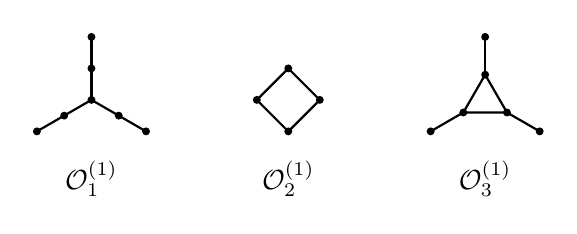
\begin{tikzpicture}[thick,scale=0.5]
\tikzstyle{sommet}=[circle, draw, fill=black, inner sep=0pt, minimum width=2pt]
          
\begin{scope}[xshift=0cm,yshift=0cm,scale=0.8]
\node (v) at (0:0){};
\draw (v) node[sommet]{};
\foreach \i in {1,2}{
	\node (u\i) at (90:\i){};
	\draw (u\i) node[sommet]{};
	\node (v\i) at (210:\i){};
	\draw (v\i) node[sommet]{};
	\node (w\i) at (330:\i){};
	\draw (w\i) node[sommet]{};
	}
\draw (v.center) -- (u1.center) -- (u2.center);
\draw (v.center) -- (v1.center) -- (v2.center);
\draw (v.center) -- (w1.center) -- (w2.center);

\node[] (0) at (0,-2.5){$\mathcal{O}^{(1)}_1$};

\end{scope}
	
\begin{scope}[xshift=5cm,yshift=0cm,scale=0.8]
\foreach \i in {0,1,2,3}{
	\node (u\i) at (90*\i:1){};
	\draw (u\i) node[sommet]{};
	}
\draw (u0.center) -- (u1.center) -- (u2.center) -- (u3.center) -- (u0.center);

\node[] (0) at (0,-2.5){$\mathcal{O}^{(1)}_2$};
\end{scope}
	
\begin{scope}[xshift=10cm,yshift=0cm,scale=0.8]
\foreach \i in {0,1,2}{
	\node (u\i) at (90+120*\i:0.8){};
	\draw (u\i) node[sommet]{};
	}
\foreach \i in {0,1,2}{
	\node (v\i) at (90+120*\i:2){};
	\draw (v\i) node[sommet]{};
	}

\draw (u0.center) -- (u1.center) -- (u2.center)  -- (u0.center);
\draw (u0.center) -- (v0.center) ;
\draw (u1.center) -- (v1.center) ;
\draw (u2.center) -- (v2.center) ;

\node[] (0) at (0,-2.5){$\mathcal{O}^{(1)}_3$};
\end{scope}
	
\end{tikzpicture}

\end{document}